\begin{figure}[tbp]
\centering
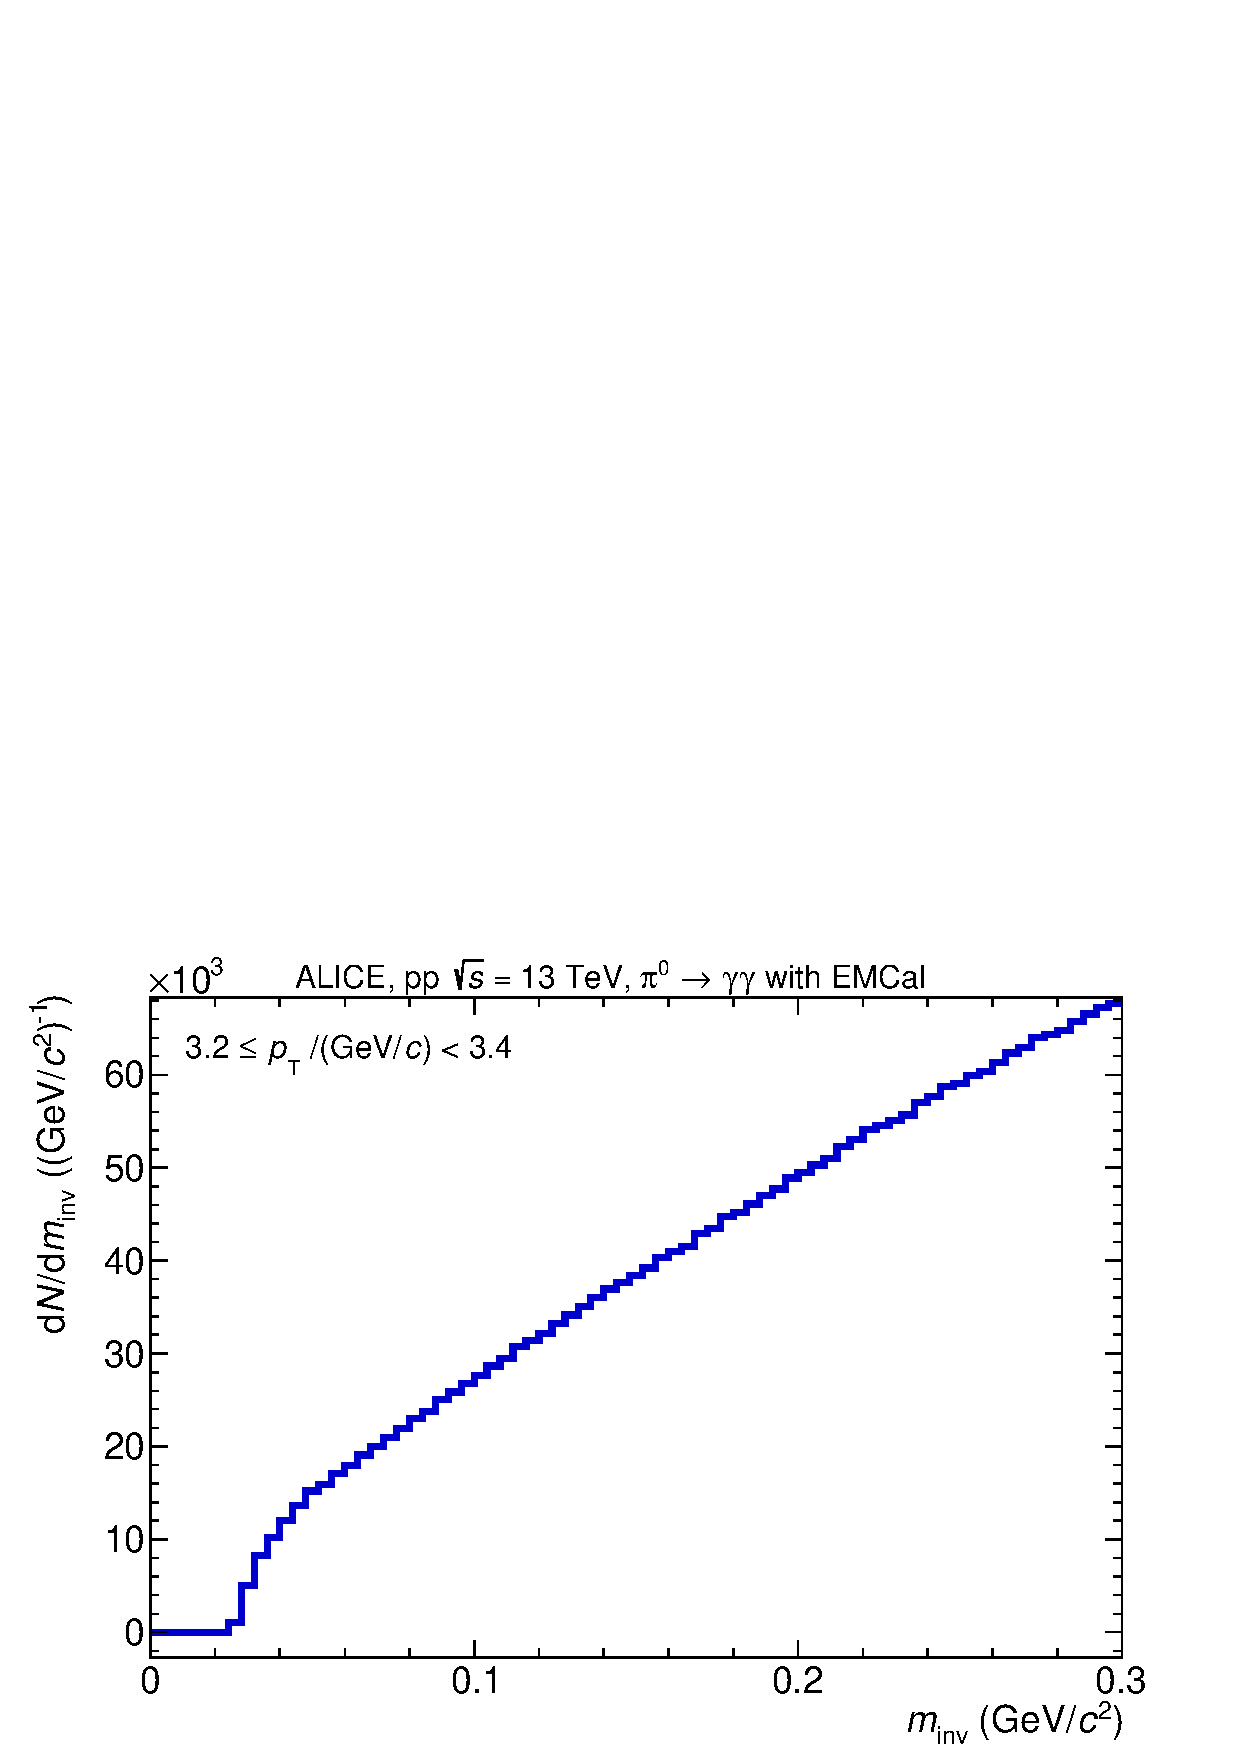
\includegraphics[width=.7\linewidth]{hUncorrBkg.pdf}
\caption{Kombinationen von Photonenkandidaten aus unterschiedlichen Kollisionen, die keine Korrelationen zueinander haben, weshalb auch kein Peak im Bereich der $\pi^{0}$-Masse zu sehen ist. Dies dient als Grundlage zur Bestimmung des unkorrelierten Untergrunds.}
\label{figUncorrBkg}
\end{figure}

	Durch das kombinieren aller Photonenkandidaten ist ein gro{\ss}er Anteil der rekonstruierten Massen aus nicht korreliert Paaren, da die beiden Photonenkandidaten nicht zusammenh{"a}ngen {\"u}ber beispielsweise einen Zerfall. Um diesen unkorrelierten Untergrund abzuw{\"a}gen kombiniert man im sogenannten Eventmixing Photonenkandidaten aus unterschiedlichen Events zusammen, da so sicher keine Verbindung zwischen den beiden Photonenkandidaten besteht. Abbildung \ref{figUncorrBkg} stellt das Ergebnis des Eventmixings f{\"u}r einen gew{\"a}hlten Bereich dar.

	Die Verteilung aus den {\it mixed events} weist keinen Peak auf und hat eine gr{\"o}{\ss}ere Anzahl Eintr{\"a}ge, als die Verteilung aus dem selben Events (vgl. Abbildung \ref{figSignalPlusBkg} und \ref{figUncorrBkg}), weshalb die mixed Event Verteilung an die der same Events skaliert werden muss. Die Skalierung erfolgt im rechten Bereich au{\ss}erhalb des $\pi^{0}$-Peaks und es ergibt sich f{\"u}r den Skalierungsfaktor:
	\begin{align}
	\label{eqBackSkalierung}
	\alpha &= \frac{\sum_{i \neq j}\sum_{n}m_{\text{inv}}\left( \gamma^{(n)}_{i},\gamma^{(n)}_{j}\right) }{\sum_{i,j}\sum_{n \neq m}m_{\text{inv}}\left( \gamma^{(n)}_{i},\gamma^{(m)}_{j}\right) }
	\end{align}
	Die oberen Indizes stehen hierbei f{\"u}r das Event, aus dem ein Photon kommt.\newline
	\begin{figure}[tbp]
		\centering
		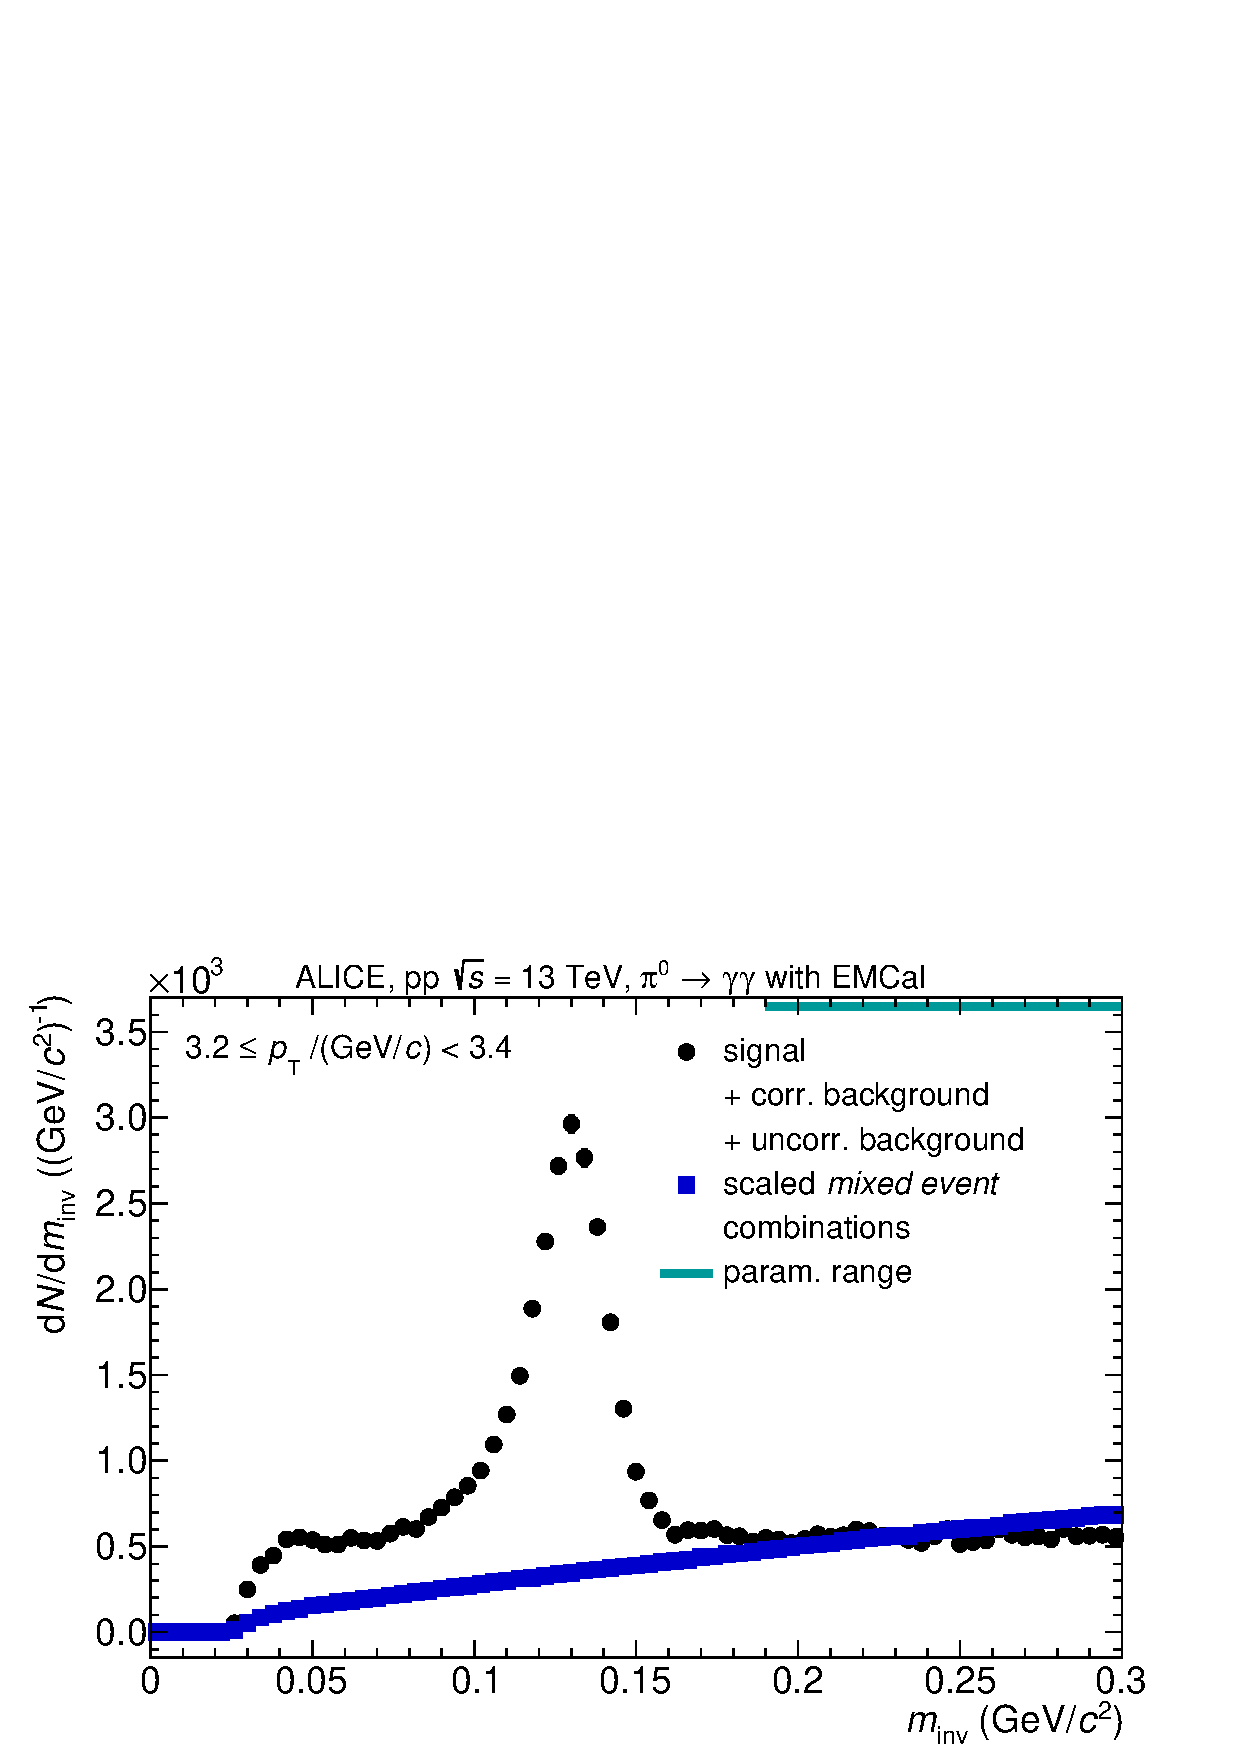
\includegraphics[width=.7\linewidth]{hUncorrBkgNorm.pdf}
		\caption{Nach Gleichung \ref{eqBackSkalierung} skalierte {\it mixed event} Rekombinationen aus Abbildung \ref{figUncorrBkg} als Absch{\"a}tzung des unkorrelierten Untergrunds zusammen aufgetragen mit Signal zuz{\"u}glich beiden Untergrundkomponenten (Abbildung \ref{figSignalPlusBkg}).}
		\label{figUncorrBkgNorm}
	\end{figure}
	Das Resultat der Skalierung ist in Abbildung \ref{figUncorrBkgNorm} zu sehen, wo zus{\"a}tzlich noch das Signal inklusiver beider Untergr{\"u}nde eingezeichnet ist, um besser erkennen zu k{\"o}nnen, wie sich der abgesch{\"a}tzte korrelierte Untergrund relativ zum gesamten Signal verh{\"a}lt.
	Das es sich hierbei nur um eine Absch{\"a}tzung handelt kann daran ausmachen werden, dass um $m_{\text{inv}} = 0,3 (\text{GeV/}c)$ der unkorrelierte Untergrund gr{\"o}{\ss}er ist, als das Signal mit beiden Untergrundkomponenten, was bedeutet, dass nach Abzug des unkorrelierten Untergrunds das Signal mit korreliertem Untergrund dort negativ w{\"a}re, was physikalisch nicht sinnvoll ist.